Jedes Minispiel ist aus drei Leveln aufgebaut, welche progressiv schwerer werden.
So dient das erste Level als Einführung in die Mechaniken des jeweiligen Minispiels.
Das zweite Level kann als \glqq standard\grqq{}-Schwierigkeitsgrad verstanden werden und im Dritten können die Spielenden dann ihre erlernten Fähigkeiten in schwierigen Herausforderungen unter Beweis stellen.
Nach dem erfolgreichen Beenden eines Levels erhält die Spielfigur ein Item, welches dann im Kampf verwendet werden kann.
Diese Items hängen von der Fachschaft und dem Schwierigkeitsgrad ab.
Die Stärke der Items skaliert also mit der Schwierigkeit des beendeten Levels. 
Da das Bearbeiten schwererer Level länger dauert, wird dies dementsprechend belohnt.\\
Im Allgemeinen soll jedes Minispiel mit einer Auswahl des Schwierigkeitsgrades beginnen, welche auch wieder verlassen werden kann, wenn sich doch gegen das Spielen entschieden wird.
Jedes Level bietet zusätzlich noch die Möglichkeit, zur Auswahl zurückzukehren.
Nach dem Abschließen des selbigen ist es ebenfalls möglich, das Level neu zu starten.


\subsection{Informatik}

Grundlegende Idee dieses Minispiels ist das \glqq Bauen\grqq{} eines Schaltkreises aus vorgegeben Logikgattern, der vorgegebene Bedingungen erfüllen soll.
Die Spielenden haben gewonnen, wenn das richtige beziehungsweise die richtigen Gatter ausgewählt wurden.
Es kann nur das erste Level verloren werden, worauf später noch eingegangen wird.\\
Die Level der Fachschaft Informatik bestehen jeweils aus zwei wesentlichen Komponenten:
Zunächst gibt es einen Schaltkreis, welcher aus Tastern, mit \glqq{}?\grqq{} verdeckten Logikgattern sowie Lämpchen aufgebaut ist.
Die zweite Komponente bilden verschiedene Logikgatter, aus welchen das im Schaltkreis verdeckte bzw. die im Schaltkreis verdeckten ausgewählt werden müssen.

\begin{figure}[H]
	\centering
	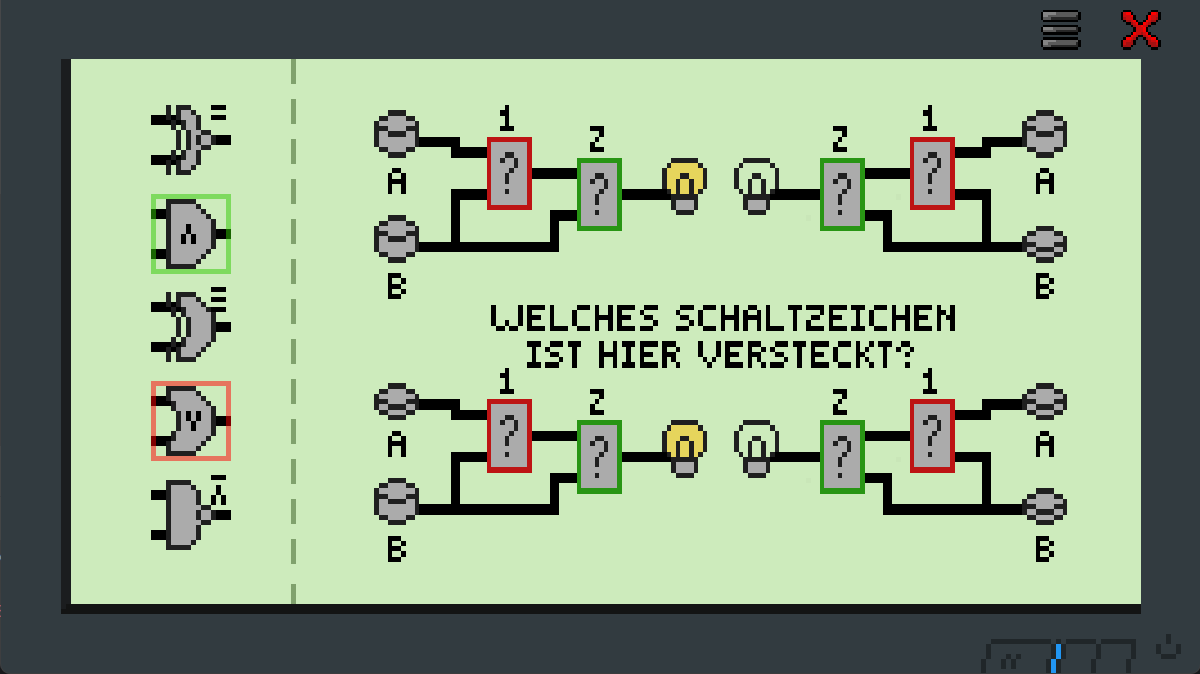
\includegraphics[width=.7\textwidth]{bilder/MinispielInformatik.png}
	\caption{Level 2 des Minispiels der Fachschaft Informatik}
	\label{fig:mginf}
\end{figure}

Verschiedene Schwierigkeiten werden auf zwei Weisen ermöglicht:

\begin{itemize}
    \item Die Anzahl an Logikgattern, aus denen ausgewählt werden kann, erhöht sich mit jedem Schwierigkeitsgrad.
            So sind es im ersten Level 4, im zweiten Level 5 und im dritten Level 6 Logikgatter, welche zur Auswahl stehen.
    \item Die Komplexität des Schaltkreises sowie die Anzahl an verdeckten Gattern ändern sich dem Schwierigkeitsgrad entsprechend.
\end{itemize}

Jedes Level verwendet außerdem, im Sinne der Variabilität, drei verschiedene Schaltkreise, aus denen bei jedem Minispiel-Start einer zufällig gewählt wird.

\subsubsection{Level 1}

Bei den Schaltkreisen des ersten Levels fehlt jeweils nur ein Logikgatter, das zwei Eingänge mit einem Ausgang verbindet.
Gesucht wird also das Logikgatter $G \in \{\land , \lor , \overline{\land}, \overline{\lor}, \veebar, \overline{\veebar}\}$\footnote{$\land = AND,\ \lor = OR,\ \overline{\land} = NAND,\ \overline{\lor} = NOR,\ \veebar = XOR,\ \overline{\veebar} = XNOR$}, welches folgende Bedingungen erfüllt:

\begin{align*}
    x_1 G x_2 = y
\end{align*}

Dadurch, dass jeder Schaltkreis zwei Eingänge und einen Ausgang besitzt, ergeben sich vier mögliche Zustände, die in Form einer Wahrheitswerttabelle dargestellt werden können.
Für die Rätsel des ersten Levels wurden folgende Tabellen festgelegt:

\begin{table}[H]
    \centering
    \begin{minipage}{.33\textwidth}
        $G = \land$\\
        \vfill
        \begin{tabular}{|c|c|c|} 
            \hline
            $x_1$ & $x_2$ & $y$ \\
            \hline\hline
            $0$ & $0$ & $0$ \\
            $0$ & $1$ & $0$ \\
            $1$ & $0$ & $0$ \\
            $1$ & $1$ & $1$ \\
            \hline
        \end{tabular}
    \end{minipage}
    \hfill
    \begin{minipage}{.32\textwidth}
        $G = \lor$\\
        \vfill
        \begin{tabular}{|c|c|c|} 
            \hline
            $x_1$ & $x_2$ & $y$ \\
            \hline\hline
            $0$ & $0$ & $0$ \\
            $0$ & $1$ & $1$ \\
            $1$ & $0$ & $1$ \\
            $1$ & $1$ & $1$ \\
            \hline
        \end{tabular}
    \end{minipage}
    \hfill
    \begin{minipage}{.33\textwidth}
        $G = \overline{\land}$\\
        \vfill
        \begin{tabular}{|c|c|c|} 
            \hline
            $x_1$ & $x_2$ & $y$ \\
            \hline\hline
            $0$ & $0$ & $1$ \\
            $0$ & $1$ & $1$ \\
            $1$ & $0$ & $1$ \\
            $1$ & $1$ & $0$ \\
            \hline
        \end{tabular}
    \end{minipage}
    \caption{Wahrheitswerttabellen für Level 1 des Informatik-Minispiels}
    \label{tab:wwt01}
\end{table}

Diese Tabellen werden den Spielenden, aufgrund der ansprechenderen Gestaltung, in Form einer Abbildung präsentiert, welche die vier Zustände des Schaltkreises darstellt.
Ebenfalls im Sinne der Gestaltung wurde auf die Konvention, die Eingänge auf der linken Seite und die Ausgänge auf der rechten Seite darzustellen, verzichtet.
In der Abbildung \ref{fig:mginf} ist dies beispielhaft anhand eines Rätsels des zweiten Levels zu erkennen.

Dieses Level kann durch das Auswählen eines falschen Gatters verloren werden, das heißt das Minispiel muss neu gestartet werden, um das Lösen durch Raten zu verhindern.
Bei den folgenden Leveln ist dies nicht der Fall, da diese schon komplex genug sind, um Raten zu verhindern.
Ein Verlieren bei Falschauswahl würde das Spielerlebnis nur verschlechtern, da dies hier eher versehentlich geschieht.
\subsubsection{Level 2}

Im zweiten Level bestehen die Schaltkreise ebenfalls aus zwei Eingängen, sowie einem Ausgang.
Der Unterschied zu Level 1 besteht hierbei darin, dass zwei Logikgatter entfernt wurden.
Durch das erste werden beide Eingänge verbunden.
Der dadurch resultierende Ausgang wird im zweiten Logikgatter wieder mit einem der Eingänge verbunden, wodurch der finale Ausgang entsteht.
Außerdem wurde zur Reduzierung der Komplexitität die Einschränkung hinzugefügt, dass sich die Gatter unterscheiden müssen.
Gesucht werden also die Logikgatter $G_1, G_2 \in \{\land , \lor , \overline{\land}, \overline{\lor}, \veebar, \overline{\veebar}\}$, welche folgende Bedingungen erfüllen:

\begin{align*}
    (x_1 G_1 x_2) G_2 x_2 &= y\\
    G_1 &\neq G_2
\end{align*}

Dadurch, dass jeder Schaltkreis auch im zweiten Level zwei Eingänge und einen Ausgang besitzt, ergeben sich wieder vier mögliche Zustände, die in Form einer Wahrheitswerttabelle dargestellt werden können.
Für die Rätsel des zweiten Levels wurden folgende Tabellen festgelegt:

\begin{table}[h!]
    \centering
    \begin{minipage}{.33\textwidth}
        $G_1 = \land$\\
        $G_2 = \overline{\lor}$
        \vfill
        \begin{tabular}{|c|c|c|} 
            \hline
            $x_1$ & $x_2$ & $y$ \\
            \hline\hline
            $0$ & $0$ & $1$ \\
            $0$ & $1$ & $0$ \\
            $1$ & $0$ & $1$ \\
            $1$ & $1$ & $0$ \\
            \hline
        \end{tabular}
    \end{minipage}
    \hfill
    \begin{minipage}{.32\textwidth}
        $G_1 = \lor$\\
        $G_2 = \veebar$
        \vfill
        \begin{tabular}{|c|c|c|} 
            \hline
            $x_1$ & $x_2$ & $y$ \\
            \hline\hline
            $0$ & $0$ & $0$ \\
            $0$ & $1$ & $0$ \\
            $1$ & $0$ & $1$ \\
            $1$ & $1$ & $0$ \\
            \hline
        \end{tabular}
    \end{minipage}
    \hfill
    \begin{minipage}{.33\textwidth}
        $G_1 = \overline{\land}$\\
        $G_2 = \lor$
        \vfill
        \begin{tabular}{|c|c|c|} 
            \hline
            $x_1$ & $x_2$ & $y$ \\
            \hline\hline
            $0$ & $0$ & $1$ \\
            $0$ & $1$ & $1$ \\
            $1$ & $0$ & $1$ \\
            $1$ & $1$ & $1$ \\
            \hline
        \end{tabular}
    \end{minipage}
    \caption{Wahrheitswerttabellen für Level 2 des Informatik-Minispiels}
    \label{tab:wwt02}
\end{table}

Diese Tabellen werden analog zu Level 1 als Abbildungen dargestellt.

\subsubsection{Level 3}

Im dritten Level bestehen die Schaltkreise aus drei Eingängen, einem Ausgang und drei entfernten Logikgattern.
Durch die ersten beiden werden jeweils zwei der Eingänge miteinander verbunden.
Die dadurch resultierenden Ausgänge werden im dritten Logikgatter verbunden, wodurch der finale Ausgang entsteht.
Gesucht werden also die Logikgatter $G_1, G_2, G_3 \in \{\land , \lor , \overline{\land}, \overline{\lor}, \veebar, \overline{\veebar}\}$, welche folgende Bedingungen erfüllen:

\begin{align*}
    (x_1 G_1 x_2) G_3 (x_2 G_2 x_3) &= y\\
    G_1 \neq G_2 &\neq G_3 
\end{align*}

Dadurch, dass jeder Schaltkreis aus drei Eingänge und einen Ausgang besteht, ergeben sich insgesamt acht mögliche Zustände, die in Form einer Wahrheitswerttabelle dargestellt werden können.
Für die Rätsel des dritten Levels wurden folgende Tabellen festgelegt:

\begin{table}[h!]
    \centering
    \begin{minipage}{.33\textwidth}
        $G_1 = \land$\\
        $G_2 = \veebar$\\
        $G_3 = \lor$
        \vfill
        \begin{tabular}{|c|c|c|c|} 
            \hline
            $x_1$ & $x_2$ & $x_3$ & $y$\\
            \hline\hline
            $0$ & $0$ & $0$ & $0$\\
            $0$ & $0$ & $1$ & $1$\\
            $0$ & $1$ & $0$ & $1$\\
            $0$ & $1$ & $1$ & $0$\\
            $1$ & $0$ & $0$ & $0$\\
            $1$ & $0$ & $1$ & $1$\\
            $1$ & $1$ & $0$ & $1$\\
            $1$ & $1$ & $1$ & $1$\\
            \hline
        \end{tabular}
    \end{minipage}
    \hfill
    \begin{minipage}{.32\textwidth}
        $G_1 = \overline{\veebar}$\\
        $G_2 = \land$\\
        $G_3 = \lor$
        \vfill
        \begin{tabular}{|c|c|c|c|} 
            \hline
            $x_1$ & $x_2$ & $x_3$ & $y$\\
            \hline\hline
            $0$ & $0$ & $0$ & $1$\\
            $0$ & $0$ & $1$ & $1$\\
            $0$ & $1$ & $0$ & $0$\\
            $0$ & $1$ & $1$ & $1$\\
            $1$ & $0$ & $0$ & $0$\\
            $1$ & $0$ & $1$ & $0$\\
            $1$ & $1$ & $0$ & $1$\\
            $1$ & $1$ & $1$ & $1$\\
            \hline
        \end{tabular}
    \end{minipage}
    \hfill
    \begin{minipage}{.33\textwidth}
        $G_1 = \veebar$\\
        $G_2 = \lor$\\
        $G_3 = \land$
        \vfill
        \begin{tabular}{|c|c|c|c|} 
            \hline
            $x_1$ & $x_2$ & $x_3$ & $y$\\
            \hline\hline
            $0$ & $0$ & $0$ & $0$\\
            $0$ & $0$ & $1$ & $0$\\
            $0$ & $1$ & $0$ & $1$\\
            $0$ & $1$ & $1$ & $1$\\
            $1$ & $0$ & $0$ & $0$\\
            $1$ & $0$ & $1$ & $1$\\
            $1$ & $1$ & $0$ & $0$\\
            $1$ & $1$ & $1$ & $0$\\
            \hline
        \end{tabular}
    \end{minipage}
    \caption{Wahrheitswerttabellen für Level 3 des Informatik-Minispiels}
    \label{tab:wwt03}
\end{table}

Da die Wahrheitswerttabellen des dritten Levels acht Zustände beinhalten, wird auf die Darstellung jedes einzelnen Zustandes verzichtet und nur der erste Zustand als Schaltkreis abgebildet.
Die anderen werden als Tabelle präsentiert.

\subsubsection{Reflexion}

Bei dem Minispiel der Fachschaft Informatik wird die Theorie spielerisch mit der Praxis verbunden.
Die Spielenden werden mit abstrakten boolschen Operationen sowie mit erwarteten Ergebnissen konfrontiert und können ihre Überlegungen dann anhand von Logikgattern und Schaltkreisen in die Tat umsetzten.
Es fördert vor allem logisches Denken, jedoch auch die Fähigkeit, mit begrenzten Mitteln ein gewünschtes Ergebnis zu erziehlen.
Außerdem regen die Rätsel durch ihre Komplexitität dazu an, Lösungsstrategien zu entwickeln, anstatt Antwortmöglichkeiten einfach auszuprobieren oder gar zu raten.\\
Das erste Level bietet einen guten Einstieg in die Funktionsweise des Spieles, da hier nur die Eigenschaften der einzelnen Gatter abgefragt und diese noch nicht verkettet werden.
Der Schwierigkeitsgrad nimmt im zweiten Level deutlich zu, jedoch kann hier durch Überlegungen, die zur Vereinfachungen des Problemes führen\footnote{Beispielsweise folgende Aussage: \glqq Der Ausgang ist in jedem Fall gleich Eingang 1.\grqq} dennoch gut eine Lösung gefunden werden.
Das dritte Level ist sehr komplex.
Es verlangt das Verbinden dreier Gatter miteinander, was definitiv über den Rahmen eines schnellen Minispiels hinausreicht.
Hier kann zwar analog zu Level 2 vereinfacht werden, jedoch bleibt das Problem dadurch dennoch sehr schwierig.
Eine Mögliche Lösung wäre das Vorgeben eines oder mehrerer Gatter, ähnlich zum in \ref{sec:mathematics} beschriebenen Mathe-Minispiel.
Auch denkbar wäre eine Einschränkung der Antwortmöglichkeiten.
So könnten die richtigen Gatter schon gegeben sein, müssten jedoch noch an die richtige Stelle plaziert werden.\\
Das Minispiel birgt neben der Schwierigkeit auch anderweitig Potential zur Verbesserung.
Die Grafiken der Logikgatter sind schwer zuzuordnen und setzten die Kenntnis ihrer Funktionsweise vorraus.
Dies könnte mit kleinen Erklärtexten oder Beispielabbildungen behoben werden.
Zusätzlich ist das wiederholte Spielen nur begrenzt möglich.
Zwar bieten die verschiedenen Schaltkreise Variabilität, jedoch ist diese aufgrund der Menge an Rätseln sehr eingeschränkt.
Die insgesamt neun Schaltkreise können schnell auswendig gelernt werden, wodurch das Spiel seine Tiefe verliert.
Dies könnte möglicherweise mit zufällig generierten Wahrheitswerttabellen behoben werden.
Jedoch ist dabei zu beachten, dass viele Tabellen keine oder mehrere Lösungen für den gegebenen Aufbau besitzen.
Es würde sich eher anbieten das Grundkonzept zu überarbeiten, da dieses generell wenig Variabilität bietet.

\subsection{Mathematik}
\label{sec:mathematics}

Die grundlegende Idee dieses Minispiels basiert auf dem chinesischen Legespiel \glqq Tangram\grqq\footnote{Seite „Tangram“. In: Wikipedia - Die freie Enzyklopädie. Bearbeitungsstand: 17. Januar 2025, 11:35 UTC. URL: https://de.wikipedia.org/w/index.php?title=Tangram\&oldid=252340816 (Abgerufen: 14. April 2026, 11:30 UTC)}.
Hierbei wird versucht aus gegebenen Steinen eine gegebene Form zu legen.
Die Spielenden haben gewonnen, wenn die Form zu 97.5\% mit Steinen bedeckt ist, um das Spielerlebnis angenehmer zu gestalten, da die Steine so nicht exakt am richtigen Platz liegen müssen.
Diese Überprüfung soll automatisch beim Platzieren der Steine ablaufen, um so das Drücken eines \glqqÜberprüfungs\grqq{}-Knopfes zu ersparen.
Das Minispiel kann nicht verloren werden.\\
Die Level der Fachschaft Mathematik bestehen ebenfalls aus zwei wesentlichen Komponenten:
Zunächst gibt es einen Satz an Tangram-Steinen, welche durch Verschieben und Rotieren in eine vorgegebene Silhouette, welche die zweite Komponente darstellt, gelegt werden müssen.
Außerdem werden zufällig gewählte Steine bereits an die richtige Position platziert, um das Lösen zu vereinfachen.

\begin{figure}[H]
	\centering
	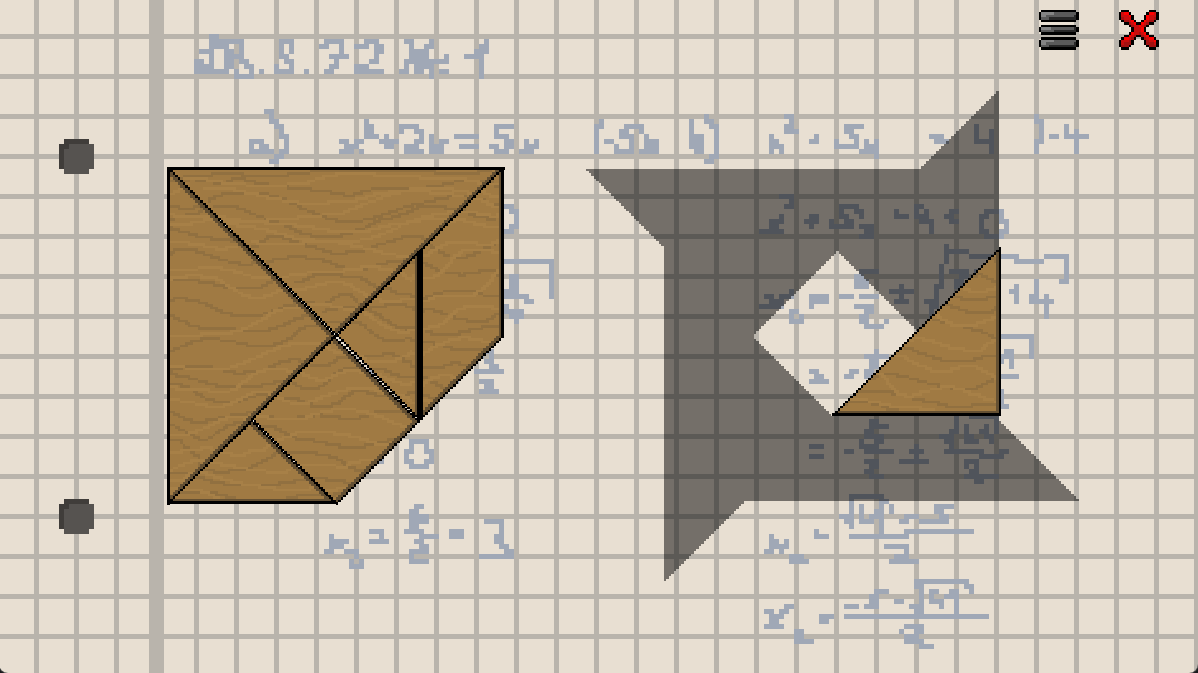
\includegraphics[width=.7\textwidth]{bilder/MinispielMathematik.png}
	\caption{Level 2 des Minispiels der Fachschaft Mathematik}
	\label{fig:mgma}
\end{figure}


Verschiedene Schwierigkeiten werden auf zwei Weisen ermöglicht:

\begin{itemize}
    \item Die Anzahl an bereits richtig angeordneten Tangram-Steinen, verringert sich mit jedem Schwierigkeitsgrad.
            So sind es im ersten Level zwei vorgegebene Steine, im zweiten Level ein und im dritten Level kein vorgegebener Stein.
    \item Die Komplexitität der Silhouette ändert sich dem Schwierigkeitsgrad entsprechend.
\end{itemize}

Jedes Level verwendet außerdem, im Sinne der Variabilität, drei verschiedene Silhouetten, aus denen bei jedem Minispiel-Start eine zufällig gewählt wird.

\subsubsection{Level 1}

Im folgenden sind die Puzzle des ersten Levels mit einer beispielhaften Lösung abgebildet.

\begin{figure}[H]
    \centering
    \begin{minipage}{0.33\textwidth}
        
\includegraphics[width=1\textwidth]{bilder/TangramHerz.png}
        \caption{Herz}
        \label{fig:therz}
    \end{minipage}
    \hfill
    \begin{minipage}{0.32\textwidth}
        
\includegraphics[width=1\textwidth]{bilder/TangramSchwan.png}
        \caption{Schwan}
        \label{fig:tschwan}
    \end{minipage}
    \hfill
    \begin{minipage}{0.33\textwidth}
        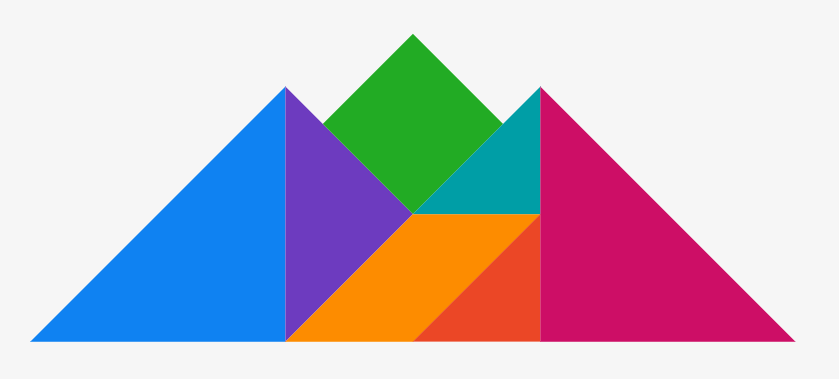
\includegraphics[width=1\textwidth]{bilder/TangramBerg.png}
        \caption{Berg}
        \label{fig:tberg}
    \end{minipage}
\end{figure}

\subsubsection{Level 2}

Im folgenden sind die Puzzle des zweiten Levels mit einer beispielhaften Lösung abgebildet.

\begin{figure}[H]
    \centering
    \begin{minipage}{0.33\textwidth}
        
\includegraphics[width=1\textwidth]{bilder/TangramHaus.png}
        \caption{Haus}
        \label{fig:thaus}
    \end{minipage}
    \hfill
    \begin{minipage}{0.32\textwidth}
        
\includegraphics[width=1\textwidth]{bilder/TangramNinjastern.png}
        \caption{Ninjastern}
        \label{fig:tninjastern}
    \end{minipage}
    \hfill
    \begin{minipage}{0.33\textwidth}
        
\includegraphics[width=1\textwidth]{bilder/TangramBaum.png}
        \caption{Baum}
        \label{fig:tbaum}
    \end{minipage}
\end{figure}

\subsubsection{Level 3}

Im folgenden sind die Puzzle des dritten Levels mit einer beispielhaften Lösung abgebildet.

\begin{figure}[H]
    \centering
    \begin{minipage}{0.33\textwidth}
        
\includegraphics[width=1\textwidth]{bilder/TangramLäufer.png}
        \caption{Läufer}
        \label{fig:tlaeufer}
    \end{minipage}
    \hfill
    \begin{minipage}{0.32\textwidth}
        
\includegraphics[width=1\textwidth]{bilder/TangramKamel.png}
        \caption{Kamel}
        \label{fig:tkamel}
    \end{minipage}
    \hfill
    \begin{minipage}{0.33\textwidth}
        
\includegraphics[width=1\textwidth]{bilder/TangramHai.png}
        \caption{Hai}
        \label{fig:thai}
    \end{minipage}
\end{figure}

\subsubsection{Reflexion}

Das Minispiel der Fachschaft Mathematik nutz das seit Jahrhunderten bewährte chinesische Legespiel \glqq Tangram\grqq{} um das räumliche Denken der Spielenden auf die Probe zu stellen.
Es mag sehr simpel erscheinen, besitzt jedoch viele mathematische Rafinessen, welche teilweise auch in unserem Schulhaus beleuchtet werden. 
Es fördert neben dem bereits Genannten ebenfalls die Fähigkeit Strukturen zu erkennen und diese zu verallgemeinern.
Die meißten Tangramsteine können als eine Kombination anderer dargestellt werden, wodurch sowohl Vielfalt als auch Restriktion entsteht.
Sollte beispielsweise ein großer Stein übrig sein, jedoch nur kleine freie Plätze, kann versucht werden bereits platzierte Steine durch den Übrigen zu ersetzten und mit den frei gewordenen Steinen die Lücken zu füllen.\\
Die einzelnen Level unterscheiden sich wenig voneinander.
Die Schwierigkeit des Lösens eines einzelnen Puzzles ist sehr subjektiv und lässt sich so schwer festlegen, weswegen die Zuteilung der Puzzle zu den jeweilligen Level nicht sinnvoll ist.
Besser wäre es diese Levelübergreifend zu definieren und so die Schwierigkeit nur durch die Anzahl der vorgegebenen Steine zu differenzieren.
Jedoch wirft auch dies Probleme auf:
Die Schwierigkeitsänderung zwischen den Leveln ist eher gering.
So kann es beispielsweise vorkommen, dass der im zweiten Level bereits platzierte Stein so gegeben ist, dass die Platzierung eines zweiten offensichtlich erscheint\footnote{Beispielsweise das Quadrat in Abbildung \ref{fig:tninjastern}, welches die Platzierung des orangenen Dreiecks vorgeben würde.}, wodurch das Lösen des Puzzles nicht schwerer, als im ersten Level ist.
Außerdem ist diese Art des Erschwerens nicht beliebig skalierbar, da nicht weniger als kein Stein vorgegeben werden kann.\\
Das dritte Level entspricht nicht vollständig dem Bild einer schwierigen Herausforderung, weil es sich, wie bereits genannt, wenig von den anderen Leveln unterscheidet und das Lösen auch etwas zu einfach ist.
Es müsste also erschwert werden, was durch das aktuelle System nicht gewährleistet werden kann.
Eine mögliche Lösung wäre das Einführen eines zweiten Tangram-Sets, wodurch deutlich komplexere Figuren möglich werden und so auch der Unterschied zu den vorherigen Schwierigkeitsgraden deutlich wird.

\subsection{Physik}
Das Physik-Minigame greift grundlegende Konzepte der klassischen Mechanik auf. Der Spieler steuert einen Ball, indem er vor dem Schuss einen Kraftpfeil vom Ball wegzieht und damit die Startgeschwindigkeit festlegt. Nach einem Klick auf \glqq{}Simulate\grqq{} fliegt der Ball unter dem Einfluss verschiedener Beschleunigungskräfte – darunter Schwerkraft und levelspezifische Driftkräfte – und soll ein grün markiertes Zielfeld treffen.

Die Spielmechanik basiert auf dem Prinzip der Überlagerung von Kräften: Die vom Spieler eingestellte Anfangskraft addiert sich pro Frame mit den Basisbeschleunigungen des Levels, was eine realistische Wurfparabel erzeugt. Trifft der Ball das Ziel, gewinnt der/die Spieler*in; fliegt er aus dem Spielfeld oder kollidiert er mit einer Wand, verliert er/sie. Das Spiel fordert den/die Spieler*in damit auf, Kräfte intuitiv abzuschätzen und die Flugbahn gedanklich vorwegzunehmen.

\subsubsection{Level 1}
Im ersten Level wirkt ausschließlich die Schwerkraft nach unten (0, +0.15 pro Frame\textsuperscript{2}).
Der Spieler zieht den Kraftpfeil nach rechts und schießt den Ball in einem Bogen zum Ziel unten rechts.
Dieses Level dient als Einstieg und vermittelt das grundlegende Spielprinzip ohne weitere Ablenkung.

\subsubsection{Level 2}
Das zweite Level ergänzt die Schwerkraft um einen leichten Drift nach links (-0.05, 0).
Der Ball wird also während des Fluges kontinuierlich nach links gezogen, was den Spieler zwingt, die Anfangskraft nach rechts entsprechend stärker einzustellen, um diesen Effekt zu kompensieren.
Die Herausforderung liegt im Abschätzen der Gesamtkraft aus zwei überlagerten Vektoren.

\subsubsection{Level 3}
Im dritten und schwersten Level wirkt ein starker Drift nach rechts (+0.12, 0) zusätzlich zur Schwerkraft.
Eine Wand blockiert den direkten Weg zum Ziel.
Der Spieler kann den Ball nur nach oben schießen und muss ihn so über die Wand hinweglenken, dass der Rechtsdrift ihn anschließend zum Ziel trägt.
Dies erfordert präzises räumliches Denken und ein Verständnis der kombinierten Kraftwirkung.

\subsubsection{Beispielcode}
Im folgenden Code werden die physikalische Grundkonzepte (Beschleunigung, Position, Kollision) festgelegt.

\begin{lstlisting}[language=Java, caption={Ballbewegung und Kollisionserkennung}]
private void ballBewegen() {
    // Alle levelspezifischen Beschleunigungen (z.B. Schwerkraft, Drift)
    // werden pro Frame auf die aktuelle Geschwindigkeit addiert.
    // Das erzeugt eine realistische Wurfparabel.
    for (double[] a : basisBeschleunigungen) {
        velX += a[0]; // horizontale Beschleunigung
        velY += a[1]; // vertikale Beschleunigung (positiv = nach unten)
    }

    // Die aktualisierte Geschwindigkeit wird auf die Position addiert
    ballX += velX;
    ballY += velY;

    // Kollision mit dem Spielfeldrand: Ball ist ausgeflogen -> verloren
    if (ballX + BALL_GROESSE <= 0 || ballX >= BREITE
        || ballY + BALL_GROESSE <= 0 || ballY >= HOEHE) {
        simulationStoppen(false);
        return;
    }

    // Kollision mit der Wand (nur Level 3):
    // Rechteck des Balls schneidet Rechteck der Wand -> verloren
    if (wand != null && new Rectangle((int) ballX, (int) ballY,
        BALL_GROESSE, BALL_GROESSE)
        .intersects(new Rectangle(wand[0], wand[1], wand[2], wand[3]))) {
        simulationStoppen(false);
        return;
    }

    // Kollision mit dem Ziel:
    // Rechteck des Balls schneidet Zielrechteck -> gewonnen
    if (new Rectangle((int) ballX, (int) ballY, BALL_GROESSE, BALL_GROESSE)
        .intersects(new Rectangle(
        (int) ziel[0], (int) ziel[1],
        (int) ziel[2], (int) ziel[3]))) {
        simulationStoppen(true);
    }
}
\end{lstlisting}

Dieser Ausschnitt des Codes befasst sich mit dem Einstellen von Kraftpfeilen, dies formt die grundlegende Spielerfahrung. Wie zu erkennen, sind die Pfeile Level-spezifisch.
\begin{lstlisting}[language=Java, caption={Spielerkraft per Maus-Drag einstellen}]
// Drag-Start: Maustaste wird auf dem Ball gedrueckt -> Ziehen beginnt
if (!ziehtGerade && gedrueckt && new Rectangle((int) ballX, (int) ballY,
        BALL_GROESSE, BALL_GROESSE).contains(maus)) {
    ziehtGerade = true;
}

// Solange die Maus gezogen wird, wird die Spielerkraft berechnet.
// Die Mausposition relativ zur Ballmitte wird durch den Massstab
// (Pixel pro Krafteinheit) geteilt, um die Kraft in Spieleinheiten
// umzurechnen.
if (ziehtGerade) {
    double rohX = (maus.x - mx) / (double) MASSSTAB;
    double rohY = (maus.y - my) / (double) MASSSTAB;

    if ("RIGHT".equals(kraftRichtung)) {
        // Level 1 & 2: Kraft nur nach rechts erlaubt (kein negativer X-Wert)
        spielerKraftX = Math.max(0, rohX);
        spielerKraftY = 0;
    } else {
        // Level 3: Kraft nur nach oben erlaubt (kein positiver Y-Wert,
        // da Y-Achse in Java nach unten zeigt)
        spielerKraftX = 0;
        spielerKraftY = Math.min(0, rohY);
    }
}
\end{lstlisting}

\subsubsection{Reflexion}

Das Minigame des Fachbereich Physik passt, durch den Artstyle, perfekt zum Rest des CZGame. Die bunten Farben lassen es insgesamt spaßiger wirken, bei näherem Betrachten fällt der/dem Spielenden jedoch der Hintergrund ins Auge – dort werden verschiedene Formeln des Physik gelistet, es entsteht ein Klassenraum-Feeling. Dies greift den Spielort (unser Gymnasium) erneut auf.

\textbf{Schwierigkeitsabstufung der Level} \\

Die drei Level bauen konzeptionell aufeinander auf und steigern die Komplexität gezielt. Level 1 ist bewusst einfach gehalten, wodurch das Grundprinzip des Spiels vermittelt wird. Level 2 führt eine zweite Kraft ein, die bereits ein Umdenken erfordert – der Spieler muss zwei Vektoren gleichzeitig im Kopf behalten. Level 3 kombiniert eine starke Querkraft mit einem physischen Hindernis, was die Schwierigkeit deutlich erhöht: Der Spieler kann die Kraft nur in eine Richtung einstellen und muss gleichzeitig die Wand berücksichtigen. Diese Progression fühlt sich in der Praxis fair an, da jedes Level genau eine neue Mechnik einführt. Trotz der unterschiedlichen Schwierigkeiten verändert sich die Dauer der Level jeweils um weniges, dies sorgt für kein Motivationsverlust.

\textbf{Umsetzung} \\
Die Umsetzung basiert auf einem einfachen Frame-by-Frame Physikmodell, das pro Frame Beschleunigungen auf die Geschwindigkeit und die Geschwindigkeit auf die Position addiert. Dieses Modell ist bewusst vereinfacht – es gibt keine Reibung, keine elastischen Kollisionen und keine Zeitunabhängigkeit – was für ein Minispiel aber vollkommen ausreicht. Trotz der Vereinfachungen ist die Physik nämlich logisch und nachvolziehbar.

Eine Herausforderung bei der Entwicklung war die Drag-Steuerung: Der Input-State der Engine unterscheidet zwischen PRESSED (nur ein Frame) und HELD (dauerhaft gehalten), was initial dazu führte, dass der Kraftpfeil nicht gezogen werden konnte. Erst durch die explizite Kombination beider States konnte dieses Problem gelöst werden. Zudem musste die Koordination zwischen update() und draw() sorgfältig bedacht werden, da Phasenübergänge (z.B. Simulation → Ergebnis) sonst im selben Frame verarbeitet wurden bevor sie gezeichnet werden konnten.

\subsection{Chemie}
Das Chemie-Minigame ist ein interaktives Sortierpuzzle, das strukturell dem in der Spieleentwicklung etablierten \glqq{}Water Sort\grqq{}-Prinzip folgt. Die Spielmechanik basiert auf dem Konzept des geordneten Stapels (Stack): Mehrere Reagenzgläser sind mit farbigen Blöcken unterschiedlicher Farbe befüllt, wobei die Reihenfolge der Blöcke zufällig generiert wird. Das Ziel des Spielers ist es, durch gezielte Umfülloperationen einen Zustand herzustellen, in dem jedes Reagenzglas ausschließlich Blöcke einer einzigen Farbe enthält.

Die Interaktion erfolgt ausschließlich durch Mausklicks: Der Spieler wählt zunächst ein Quellglas aus, woraufhin dieses visuell hervorgehoben wird, und wählt anschließend ein Zielglas. Eine Umfüllung wird nur dann durchgeführt, wenn die Regeln erfüllt sind — das Zielglas ist entweder leer oder der oberste Block hat dieselbe Farbe wie die zu verschiebenden Blöcke. Gleichzeitig läuft ein Countdown-Timer, der den Spieler unter Zeitdruck setzt. Dieses Design fördert strategisches Vorausdenken sowie die Fähigkeit, mehrere Züge im Voraus zu planen.
Das Kernkonzept der Implementierung ist die Modellierung jedes Reagenzglases als Stack-Datenstruktur. Die innere Klasse Reagenzglas kapselt eine ArrayList<String>, auf der ausschließlich stack-typische Operationen erlaubt sind: Hinzufügen am Ende (blockHinzufuegen), Lesen des obersten Elements (oberstenBlockAnschauen) und Entfernen des obersten Elements (oberstenBlockEntfernen). Diese strikte Kapselung stellt sicher, dass die Spielregeln strukturell durch das Datenmodell erzwungen werden und nicht nur durch externe Überprüfungen.

Die Methode kannAblegen() der Klasse Reagenzglas fasst die Ablegelogik zentral zusammen: Ein Block darf nur dann platziert werden, wenn das Glas nicht voll ist und entweder leer ist oder der oberste Block dieselbe Farbe trägt. Diese Kapselung der Regellogik im Datenmodell folgt dem Prinzip der hohen Kohäsion und verhindert, dass Spielregeln an verschiedenen Stellen im Code dupliziert werden.


\subsubsection{Level 1}

Drei Farben (Blau, Grün, Pink) werden auf drei Reagenzgläser verteilt, dazu kommen zwei leere Puffergläser. Mit insgesamt 12 Blöcken und einem großzügigen Verhältnis von Puffer- zu Spielgläsern ist dieses Level bewusst zugänglich gehalten und dient primär dem Kennenlernen der Steuerung und der Spielregeln.
\subsubsection{Level 2}
Mit vier Farben (Blau, Grün, Pink, Lila) steigt die Anzahl der Blöcke auf 16. Der Zustandsraum möglicher Anordnungen wächst kombinatorisch, sodass triviale Lösungswege nicht mehr ausreichen. Die Puffergläser müssen strategisch eingesetzt werden, was ein höheres Maß an planerischem Denken voraussetzt.
\subsubsection{Level 3}
Alle fünf Farben (Blau, Grün, Pink, Lila, Gelb) sind aktiv. 20 Blöcke auf fünf Spielgläsern bei nur zwei Puffergläsern ergeben eine deutlich erhöhte Schwierigkeit. Das Zeitlimit von 30 Sekunden ist bei dieser Komplexität besonders herausfordernd, da die Lösung typischerweise eine längere Zugsequenz erfordert.

\subsubsection{Beispielcode}
\begin{lstlisting}[language=Java, caption={Umschütten: Blöcke von einem Glas ins andere verschieben}]
private void umschuetten(int von, int nach) {
    Reagenzglas v = glaeser.get(von);
    Reagenzglas n = glaeser.get(nach);
    String farbe = v.oberstenBlockAnschauen();

    // Abbruch, wenn Quellglas leer oder Zielglas Farbe nicht annimmt
    if (farbe == null || !n.kannAblegen(farbe)) return;

    // Alle gleichfarbigen Bloecke vom Stapel verschieben (so viele wie moeglich).
    // Die Schleife verschiebt solange Bloecke, wie die Farbe uebereinstimmt
    // und das Zielglas noch Kapazitaet hat -- simuliert das physische
    // Umschuetten mehrerer Schichten auf einmal.
    while (v.oberstenBlockAnschauen() != null
            && v.oberstenBlockAnschauen().equals(farbe)
            && n.kannAblegen(farbe))
        n.blockHinzufuegen(v.oberstenBlockEntfernen());
}
\end{lstlisting}

\begin{lstlisting}[language=Java, caption={Gewinnbedingung: Prüfung ob alle Gläser gelöst sind}]
// Ein einzelnes Glas gilt als geloest, wenn es vollstaendig gefuellt
// und ausschliesslich mit einer einzigen Farbe belegt ist.
public boolean istGeloest() {
    if (bloecke.size() != MAX_KAPAZITAET) return false;
    String f = bloecke.getFirst();
    for (String b : bloecke) if (!b.equals(f)) return false;
    return true;
}

// Das Gesamtlevel ist gewonnen, wenn alle nicht-leeren Glaeser
// die Loesungsbedingung erfuellen. Leere Pufferglaeser werden
// dabei explizit ignoriert, da sie keinen Spielzustand darstellen.
private boolean istGewonnen() {
    for (Reagenzglas g : glaeser)
        if (!g.istLeer() && !g.istGeloest()) return false;
    return true;
}
\end{lstlisting}

\subsubsection{Reflexion}
\textbf{Schwierigkeitsabstufung und Spielbalance} \\
Die Progression von drei auf fünf Farben ist nicht linear, sondern exponentiell: Die Anzahl möglicher Ausgangszustände wächst mit jeder zusätzlichen Farbe kombinatorisch, da die zufällige Initialbefüllung über Collections.shuffle() jeden theoretisch erreichbaren Zustand erzeugen kann — einschließlich solcher, die eine sehr lange Lösungssequenz erfordern. In der Praxis bedeutet dies, dass Level 3 in einzelnen Durchläufen deutlich schwerer sein kann als in anderen, da die Lösbarkeit zwar stets garantiert ist (durch die zwei Puffergläser), die optimale Zugsequenz jedoch stark von der zufälligen Startanordnung abhängt. Eine mögliche Verbesserung wäre die Implementierung eines Lösbarkeits-Checks nach der Generierung, der sicherstellt, dass der Puzzlezustand innerhalb einer definierten Maximalzugzahl lösbar ist.
\textbf{Technische Umsetzung und Designentscheidungen} \\
Die Verwendung einer ArrayList als zugrundeliegende Datenstruktur für den Stack ist aus Effizienzgesichtspunkten vertretbar, da die Kapazität mit MAX\_KAPAZITAET = 4 fest begrenzt ist und keine dynamischen Resize-Operationen anfallen. Die strikte Kapselung der Stack-Operationen innerhalb der inneren Klasse Reagenzglas erhöht die Wartbarkeit des Codes erheblich, da Regeländerungen — etwa eine geänderte Kapazität oder neue Ablege-Bedingungen — ausschließlich innerhalb dieser Klasse vorgenommen werden müssen.

Eine technische Herausforderung stellte die pixelgenaue Positionierung der Blöcke innerhalb der Reagenzglas-Sprites dar. Da das Spiel mit einem festen Skalierungsfaktor (SCALE = 4) arbeitet und die Blockpositionen manuell über Pixel-Offsets (BLOCK\_X\_OFFSET, BLOCK\_BODEN\_Y) berechnet werden, ist die Darstellung eng an die konkrete Pixelart-Grafik gekoppelt. Dies stellt eine enge Kopplung zwischen Spiellogik und Asset-Design dar, die bei einer Weiterentwicklung — etwa dem Austausch der Grafiken — erneuten Anpassungsaufwand erfordern würde. Eine abstraktere Positionierungslogik, die Blockpositionen relativ zur Glasgeometrie berechnet, wäre hier langfristig robuster.
